% Options for packages loaded elsewhere
\PassOptionsToPackage{unicode}{hyperref}
\PassOptionsToPackage{hyphens}{url}
%
\documentclass[
]{article}
\usepackage{amsmath,amssymb}
\usepackage{iftex}
\ifPDFTeX
  \usepackage[T1]{fontenc}
  \usepackage[utf8]{inputenc}
  \usepackage{textcomp} % provide euro and other symbols
\else % if luatex or xetex
  \usepackage{unicode-math} % this also loads fontspec
  \defaultfontfeatures{Scale=MatchLowercase}
  \defaultfontfeatures[\rmfamily]{Ligatures=TeX,Scale=1}
\fi
\usepackage{lmodern}
\ifPDFTeX\else
  % xetex/luatex font selection
\fi
% Use upquote if available, for straight quotes in verbatim environments
\IfFileExists{upquote.sty}{\usepackage{upquote}}{}
\IfFileExists{microtype.sty}{% use microtype if available
  \usepackage[]{microtype}
  \UseMicrotypeSet[protrusion]{basicmath} % disable protrusion for tt fonts
}{}
\makeatletter
\@ifundefined{KOMAClassName}{% if non-KOMA class
  \IfFileExists{parskip.sty}{%
    \usepackage{parskip}
  }{% else
    \setlength{\parindent}{0pt}
    \setlength{\parskip}{6pt plus 2pt minus 1pt}}
}{% if KOMA class
  \KOMAoptions{parskip=half}}
\makeatother
\usepackage{xcolor}
\usepackage[margin=1in]{geometry}
\usepackage{color}
\usepackage{fancyvrb}
\newcommand{\VerbBar}{|}
\newcommand{\VERB}{\Verb[commandchars=\\\{\}]}
\DefineVerbatimEnvironment{Highlighting}{Verbatim}{commandchars=\\\{\}}
% Add ',fontsize=\small' for more characters per line
\usepackage{framed}
\definecolor{shadecolor}{RGB}{248,248,248}
\newenvironment{Shaded}{\begin{snugshade}}{\end{snugshade}}
\newcommand{\AlertTok}[1]{\textcolor[rgb]{0.94,0.16,0.16}{#1}}
\newcommand{\AnnotationTok}[1]{\textcolor[rgb]{0.56,0.35,0.01}{\textbf{\textit{#1}}}}
\newcommand{\AttributeTok}[1]{\textcolor[rgb]{0.13,0.29,0.53}{#1}}
\newcommand{\BaseNTok}[1]{\textcolor[rgb]{0.00,0.00,0.81}{#1}}
\newcommand{\BuiltInTok}[1]{#1}
\newcommand{\CharTok}[1]{\textcolor[rgb]{0.31,0.60,0.02}{#1}}
\newcommand{\CommentTok}[1]{\textcolor[rgb]{0.56,0.35,0.01}{\textit{#1}}}
\newcommand{\CommentVarTok}[1]{\textcolor[rgb]{0.56,0.35,0.01}{\textbf{\textit{#1}}}}
\newcommand{\ConstantTok}[1]{\textcolor[rgb]{0.56,0.35,0.01}{#1}}
\newcommand{\ControlFlowTok}[1]{\textcolor[rgb]{0.13,0.29,0.53}{\textbf{#1}}}
\newcommand{\DataTypeTok}[1]{\textcolor[rgb]{0.13,0.29,0.53}{#1}}
\newcommand{\DecValTok}[1]{\textcolor[rgb]{0.00,0.00,0.81}{#1}}
\newcommand{\DocumentationTok}[1]{\textcolor[rgb]{0.56,0.35,0.01}{\textbf{\textit{#1}}}}
\newcommand{\ErrorTok}[1]{\textcolor[rgb]{0.64,0.00,0.00}{\textbf{#1}}}
\newcommand{\ExtensionTok}[1]{#1}
\newcommand{\FloatTok}[1]{\textcolor[rgb]{0.00,0.00,0.81}{#1}}
\newcommand{\FunctionTok}[1]{\textcolor[rgb]{0.13,0.29,0.53}{\textbf{#1}}}
\newcommand{\ImportTok}[1]{#1}
\newcommand{\InformationTok}[1]{\textcolor[rgb]{0.56,0.35,0.01}{\textbf{\textit{#1}}}}
\newcommand{\KeywordTok}[1]{\textcolor[rgb]{0.13,0.29,0.53}{\textbf{#1}}}
\newcommand{\NormalTok}[1]{#1}
\newcommand{\OperatorTok}[1]{\textcolor[rgb]{0.81,0.36,0.00}{\textbf{#1}}}
\newcommand{\OtherTok}[1]{\textcolor[rgb]{0.56,0.35,0.01}{#1}}
\newcommand{\PreprocessorTok}[1]{\textcolor[rgb]{0.56,0.35,0.01}{\textit{#1}}}
\newcommand{\RegionMarkerTok}[1]{#1}
\newcommand{\SpecialCharTok}[1]{\textcolor[rgb]{0.81,0.36,0.00}{\textbf{#1}}}
\newcommand{\SpecialStringTok}[1]{\textcolor[rgb]{0.31,0.60,0.02}{#1}}
\newcommand{\StringTok}[1]{\textcolor[rgb]{0.31,0.60,0.02}{#1}}
\newcommand{\VariableTok}[1]{\textcolor[rgb]{0.00,0.00,0.00}{#1}}
\newcommand{\VerbatimStringTok}[1]{\textcolor[rgb]{0.31,0.60,0.02}{#1}}
\newcommand{\WarningTok}[1]{\textcolor[rgb]{0.56,0.35,0.01}{\textbf{\textit{#1}}}}
\usepackage{longtable,booktabs,array}
\usepackage{calc} % for calculating minipage widths
% Correct order of tables after \paragraph or \subparagraph
\usepackage{etoolbox}
\makeatletter
\patchcmd\longtable{\par}{\if@noskipsec\mbox{}\fi\par}{}{}
\makeatother
% Allow footnotes in longtable head/foot
\IfFileExists{footnotehyper.sty}{\usepackage{footnotehyper}}{\usepackage{footnote}}
\makesavenoteenv{longtable}
\usepackage{graphicx}
\makeatletter
\def\maxwidth{\ifdim\Gin@nat@width>\linewidth\linewidth\else\Gin@nat@width\fi}
\def\maxheight{\ifdim\Gin@nat@height>\textheight\textheight\else\Gin@nat@height\fi}
\makeatother
% Scale images if necessary, so that they will not overflow the page
% margins by default, and it is still possible to overwrite the defaults
% using explicit options in \includegraphics[width, height, ...]{}
\setkeys{Gin}{width=\maxwidth,height=\maxheight,keepaspectratio}
% Set default figure placement to htbp
\makeatletter
\def\fps@figure{htbp}
\makeatother
\setlength{\emergencystretch}{3em} % prevent overfull lines
\providecommand{\tightlist}{%
  \setlength{\itemsep}{0pt}\setlength{\parskip}{0pt}}
\setcounter{secnumdepth}{5}
\ifLuaTeX
  \usepackage{selnolig}  % disable illegal ligatures
\fi
\usepackage{bookmark}
\IfFileExists{xurl.sty}{\usepackage{xurl}}{} % add URL line breaks if available
\urlstyle{same}
\hypersetup{
  pdftitle={Week 2: Starting with R},
  pdfauthor={UZH n UU: tested by Jonas},
  hidelinks,
  pdfcreator={LaTeX via pandoc}}

\title{Week 2: Starting with R}
\author{UZH n UU: tested by Jonas}
\date{13 February, 2025}

\begin{document}
\maketitle

{
\setcounter{tocdepth}{2}
\tableofcontents
}
\section{Exercises for the R-Beginner - The fancy calculator}\label{exercises-for-the-r-beginner---the-fancy-calculator}

\subsection{Exercise 4}\label{exercise-4}

\begin{itemize}
\tightlist
\item
  from \url{https://alexd106.github.io/intro2R/exercise_4.html}
  \#task 2 is downloading data file
  \#task 3 is only reading
\end{itemize}

\#task 4

\begin{Shaded}
\begin{Highlighting}[]
\NormalTok{squid }\OtherTok{\textless{}{-}} \FunctionTok{read.table}\NormalTok{ (}\StringTok{\textquotesingle{}../data4exercises/squid1.txt\textquotesingle{}}\NormalTok{, }\AttributeTok{header=}\ConstantTok{TRUE}\NormalTok{)}
\FunctionTok{str}\NormalTok{(squid)}
\end{Highlighting}
\end{Shaded}

\begin{verbatim}
## 'data.frame':    519 obs. of  13 variables:
##  $ sample.no        : int  105128901 105128901 105128901 105128901 105128901 105128901 105128901 105128901 105128901 105128901 ...
##  $ specimen         : int  1002 1003 1005 1007 1008 1009 1011 1013 1014 1017 ...
##  $ year             : int  1989 1989 1989 1989 1989 1989 1989 1989 1989 1989 ...
##  $ month            : int  12 12 12 12 12 12 12 12 12 12 ...
##  $ weight           : num  152 106 138 141 126 ...
##  $ sex              : int  2 2 2 2 2 2 2 2 2 2 ...
##  $ maturity.stage   : int  3 1 2 2 3 1 2 3 3 4 ...
##  $ DML              : int  174 153 169 175 169 116 135 192 170 205 ...
##  $ eviscerate.weight: num  87.5 62.6 79.4 83.1 72.2 ...
##  $ dig.weight       : num  4.648 3.138 0.307 4.123 3.605 ...
##  $ nid.length       : num  39.4 24.1 39 41.4 39.8 20 14 55 44 53 ...
##  $ nid.weight       : num  2.46 0.319 1.169 1.631 2.03 ...
##  $ ovary.weight     : num  1.68 0.103 0.289 0.252 0.86 ...
\end{verbatim}

\begin{Shaded}
\begin{Highlighting}[]
\FunctionTok{summary}\NormalTok{ (squid)}
\end{Highlighting}
\end{Shaded}

\begin{verbatim}
##    sample.no            specimen         year          month       
##  Min.   :100039001   Min.   :1001   Min.   :1989   Min.   : 1.000  
##  1st Qu.:105079001   1st Qu.:1009   1st Qu.:1990   1st Qu.: 3.000  
##  Median :113099001   Median :1026   Median :1990   Median : 7.000  
##  Mean   :112499032   Mean   :1028   Mean   :1990   Mean   : 6.803  
##  3rd Qu.:121029101   3rd Qu.:1045   3rd Qu.:1991   3rd Qu.:10.000  
##  Max.   :130039001   Max.   :1076   Max.   :1991   Max.   :12.000  
##      weight           sex    maturity.stage       DML      eviscerate.weight
##  Min.   : 34.0   Min.   :2   Min.   :1.000   Min.   : 88   Min.   : 16.8    
##  1st Qu.:184.5   1st Qu.:2   1st Qu.:2.000   1st Qu.:187   1st Qu.: 97.0    
##  Median :272.0   Median :2   Median :3.000   Median :217   Median :138.0    
##  Mean   :286.8   Mean   :2   Mean   :3.355   Mean   :215   Mean   :149.4    
##  3rd Qu.:360.5   3rd Qu.:2   3rd Qu.:5.000   3rd Qu.:240   3rd Qu.:187.0    
##  Max.   :809.0   Max.   :2   Max.   :5.000   Max.   :323   Max.   :397.0    
##    dig.weight        nid.length       nid.weight      ovary.weight   
##  Min.   :  0.307   Min.   : 10.00   Min.   : 0.031   Min.   : 0.016  
##  1st Qu.:  4.705   1st Qu.: 34.00   1st Qu.: 0.863   1st Qu.: 0.429  
##  Median :  7.321   Median : 65.10   Median : 7.769   Median :10.461  
##  Mean   :  8.118   Mean   : 59.65   Mean   : 9.675   Mean   :12.564  
##  3rd Qu.: 10.028   3rd Qu.: 81.00   3rd Qu.:16.140   3rd Qu.:22.784  
##  Max.   :100.341   Max.   :430.20   Max.   :39.325   Max.   :50.230
\end{verbatim}

\begin{Shaded}
\begin{Highlighting}[]
\CommentTok{\# 519 observations and 13 variables }
\end{Highlighting}
\end{Shaded}

\begin{Shaded}
\begin{Highlighting}[]
\NormalTok{squid}\SpecialCharTok{$}\NormalTok{year }\OtherTok{\textless{}{-}} \FunctionTok{as.factor}\NormalTok{(squid}\SpecialCharTok{$}\NormalTok{year)}
\NormalTok{squid}\SpecialCharTok{$}\NormalTok{year }
\end{Highlighting}
\end{Shaded}

\begin{verbatim}
##   [1] 1989 1989 1989 1989 1989 1989 1989 1989 1989 1989 1989 1989 1990 1990 1990
##  [16] 1990 1990 1990 1990 1990 1990 1990 1990 1990 1990 1990 1990 1990 1990 1990
##  [31] 1990 1990 1990 1990 1990 1990 1990 1990 1990 1990 1990 1990 1990 1990 1990
##  [46] 1990 1990 1990 1990 1990 1990 1990 1990 1990 1990 1990 1990 1990 1990 1990
##  [61] 1990 1990 1990 1990 1990 1990 1990 1990 1990 1990 1990 1990 1990 1990 1990
##  [76] 1990 1990 1990 1990 1990 1990 1990 1990 1990 1990 1990 1990 1990 1990 1990
##  [91] 1990 1990 1990 1990 1990 1990 1990 1990 1990 1990 1990 1990 1990 1990 1990
## [106] 1990 1990 1990 1990 1990 1990 1990 1990 1990 1990 1990 1990 1990 1990 1990
## [121] 1990 1990 1990 1990 1990 1990 1990 1990 1990 1990 1990 1990 1990 1990 1990
## [136] 1990 1990 1990 1990 1990 1990 1990 1990 1990 1990 1990 1990 1990 1990 1990
## [151] 1990 1990 1990 1990 1990 1990 1990 1990 1990 1990 1990 1990 1990 1990 1990
## [166] 1990 1990 1990 1990 1990 1990 1990 1990 1990 1990 1990 1990 1990 1990 1990
## [181] 1990 1990 1990 1990 1990 1990 1990 1990 1990 1990 1990 1990 1990 1990 1990
## [196] 1990 1990 1990 1990 1990 1990 1990 1990 1990 1990 1990 1990 1990 1990 1990
## [211] 1990 1990 1990 1990 1990 1990 1990 1990 1990 1990 1990 1990 1990 1990 1990
## [226] 1990 1990 1990 1990 1990 1990 1990 1990 1990 1990 1990 1990 1990 1990 1990
## [241] 1990 1990 1990 1990 1990 1990 1990 1990 1990 1990 1990 1990 1990 1990 1990
## [256] 1990 1990 1990 1990 1990 1990 1990 1990 1990 1990 1990 1990 1990 1990 1990
## [271] 1990 1990 1990 1990 1990 1990 1990 1990 1990 1990 1990 1990 1990 1990 1990
## [286] 1990 1990 1990 1990 1990 1990 1990 1990 1990 1990 1990 1990 1990 1990 1990
## [301] 1990 1990 1990 1990 1990 1990 1990 1990 1990 1990 1990 1990 1990 1990 1990
## [316] 1990 1990 1990 1990 1990 1990 1990 1990 1990 1990 1990 1990 1990 1990 1990
## [331] 1990 1990 1990 1990 1990 1990 1990 1990 1990 1990 1990 1990 1990 1990 1990
## [346] 1991 1991 1991 1991 1991 1991 1991 1991 1991 1991 1991 1991 1991 1991 1991
## [361] 1991 1991 1991 1991 1991 1991 1991 1991 1991 1991 1991 1991 1991 1991 1991
## [376] 1991 1991 1991 1991 1991 1991 1991 1991 1991 1991 1991 1991 1991 1991 1991
## [391] 1991 1991 1991 1991 1991 1991 1991 1991 1991 1991 1991 1991 1991 1991 1991
## [406] 1991 1991 1991 1991 1991 1991 1991 1991 1991 1991 1991 1991 1991 1991 1991
## [421] 1991 1991 1991 1991 1991 1991 1991 1991 1991 1991 1991 1991 1991 1991 1991
## [436] 1991 1991 1991 1991 1991 1991 1991 1991 1991 1991 1991 1991 1991 1991 1991
## [451] 1991 1991 1991 1991 1991 1991 1991 1991 1991 1991 1991 1991 1991 1991 1991
## [466] 1991 1991 1991 1991 1991 1991 1991 1991 1991 1991 1991 1991 1991 1991 1991
## [481] 1991 1991 1991 1991 1991 1991 1991 1991 1991 1991 1991 1991 1991 1991 1991
## [496] 1991 1991 1991 1991 1991 1991 1991 1991 1991 1991 1991 1991 1991 1991 1991
## [511] 1991 1991 1991 1991 1991 1991 1991 1991 1991
## Levels: 1989 1990 1991
\end{verbatim}

\begin{Shaded}
\begin{Highlighting}[]
\NormalTok{squid}\SpecialCharTok{$}\NormalTok{month }\OtherTok{\textless{}{-}} \FunctionTok{as.factor}\NormalTok{(squid}\SpecialCharTok{$}\NormalTok{month)}
\NormalTok{squid}\SpecialCharTok{$}\NormalTok{month}
\end{Highlighting}
\end{Shaded}

\begin{verbatim}
##   [1] 12 12 12 12 12 12 12 12 12 12 12 12 1  1  1  3  3  3  3  3  3  3  3  3  3 
##  [26] 3  3  3  3  3  3  3  3  3  3  3  3  3  3  3  3  3  3  3  3  3  3  3  3  3 
##  [51] 3  3  3  3  3  4  4  4  4  4  4  4  4  4  4  5  7  7  7  7  7  7  7  7  7 
##  [76] 7  7  7  7  7  7  7  7  7  7  7  7  7  7  7  7  7  7  7  7  7  7  7  7  7 
## [101] 7  7  7  7  7  7  7  7  8  8  8  8  8  8  8  8  8  8  8  8  8  8  8  8  8 
## [126] 8  8  8  8  8  8  8  8  8  8  8  8  9  9  9  9  9  9  9  9  9  9  9  9  9 
## [151] 9  9  9  9  9  9  9  9  9  9  9  9  9  9  9  9  9  9  9  9  9  9  9  9  9 
## [176] 9  9  9  9  9  9  9  9  9  9  9  9  9  9  9  9  9  9  9  9  9  9  9  9  9 
## [201] 9  9  9  9  9  9  9  9  9  9  9  9  9  9  9  9  9  9  9  10 10 10 10 10 10
## [226] 10 10 10 10 10 10 10 10 10 10 10 10 10 11 11 11 11 11 11 11 11 11 11 11 11
## [251] 11 11 11 11 11 11 11 11 11 11 11 11 11 11 11 11 11 11 11 11 11 11 11 11 11
## [276] 11 11 11 11 11 11 11 11 11 11 11 11 11 11 11 11 11 11 11 11 11 11 11 11 11
## [301] 11 11 11 11 11 11 11 11 11 11 11 11 11 11 12 12 12 12 12 12 12 12 12 12 12
## [326] 12 12 12 12 12 12 12 12 12 12 12 12 12 12 12 12 12 12 12 12 1  1  1  1  1 
## [351] 1  1  1  1  1  1  1  1  1  1  1  1  1  1  1  1  1  1  1  1  1  1  1  1  1 
## [376] 1  1  1  1  1  1  1  2  2  2  2  2  2  2  2  2  2  2  2  2  2  2  2  2  2 
## [401] 2  2  2  2  2  2  2  2  2  2  2  2  3  3  3  3  3  3  3  3  3  3  3  3  3 
## [426] 3  3  3  3  3  3  3  3  3  3  3  3  3  3  3  3  4  4  4  4  4  4  4  4  4 
## [451] 4  4  4  4  4  4  4  4  4  4  4  4  4  4  4  4  4  4  4  4  4  4  4  4  5 
## [476] 5  5  5  5  5  5  5  5  5  5  5  5  5  5  5  5  5  5  5  5  5  5  5  5  5 
## [501] 5  5  5  5  6  6  6  6  6  6  6  6  6  6  6  6  6  6  7 
## Levels: 1 2 3 4 5 6 7 8 9 10 11 12
\end{verbatim}

\begin{Shaded}
\begin{Highlighting}[]
\NormalTok{squid}\SpecialCharTok{$}\NormalTok{maturity.stage }\OtherTok{\textless{}{-}} \FunctionTok{factor}\NormalTok{(squid}\SpecialCharTok{$}\NormalTok{maturity.stage)}
\NormalTok{squid}\SpecialCharTok{$}\NormalTok{maturity.stage}
\end{Highlighting}
\end{Shaded}

\begin{verbatim}
##   [1] 3 1 2 2 3 1 2 3 3 4 3 4 4 5 4 4 4 5 4 5 4 4 5 5 5 5 5 4 5 4 5 4 5 5 5 5 4
##  [38] 5 5 5 4 4 5 5 5 5 5 5 5 5 4 5 4 4 4 4 4 5 4 4 4 4 4 5 5 5 1 2 5 4 5 4 1 1
##  [75] 2 2 2 5 5 2 1 2 2 1 1 1 2 2 5 2 5 2 2 5 2 2 2 2 2 2 2 1 4 2 2 2 4 5 2 2 2
## [112] 2 2 2 2 4 2 2 2 2 2 3 3 2 2 3 2 2 2 4 3 4 2 3 2 2 2 2 2 2 2 2 2 2 2 2 2 2
## [149] 3 3 2 2 2 2 2 2 2 2 2 2 2 2 2 2 2 2 2 2 2 2 2 2 2 2 2 2 2 1 2 2 2 3 2 2 2
## [186] 2 2 2 2 2 2 2 2 2 2 2 2 2 2 2 2 2 3 2 2 2 2 2 2 2 2 2 2 2 2 3 2 2 2 2 2 2
## [223] 2 2 1 3 2 2 2 2 2 2 2 2 2 2 2 2 2 2 3 3 1 2 2 2 3 3 2 3 2 2 2 2 2 2 3 2 2
## [260] 2 2 2 3 3 2 2 3 3 3 2 2 2 3 3 2 2 2 3 4 3 3 3 3 3 5 3 3 3 4 4 3 4 4 2 2 4
## [297] 5 3 5 2 4 2 4 3 3 4 3 3 3 3 2 4 2 3 4 3 3 3 1 3 2 5 4 4 4 4 4 5 5 2 5 3 4
## [334] 4 4 4 4 5 5 4 4 1 2 2 3 4 5 5 4 5 4 5 4 4 5 5 3 4 4 5 4 5 4 5 5 5 4 5 4 4
## [371] 4 5 4 5 4 2 3 5 5 5 5 4 5 4 5 2 5 4 4 4 5 4 5 5 5 5 4 5 5 5 5 5 5 4 5 4 5
## [408] 5 5 5 5 5 5 4 5 5 5 5 5 4 5 5 5 4 5 5 5 5 5 5 5 5 5 4 4 5 5 5 5 4 5 5 4 4
## [445] 5 5 5 1 4 4 5 4 4 5 5 5 5 4 5 5 5 4 5 5 5 4 4 4 5 4 2 3 1 4 4 5 5 3 5 5 5
## [482] 5 5 4 5 5 5 5 5 4 5 5 5 5 5 5 5 5 5 5 4 5 4 4 1 2 2 2 2 1 2 1 1 5 5 5 4 2
## [519] 4
## Levels: 1 2 3 4 5
\end{verbatim}

\begin{Shaded}
\begin{Highlighting}[]
\FunctionTok{str}\NormalTok{(squid)}
\end{Highlighting}
\end{Shaded}

\begin{verbatim}
## 'data.frame':    519 obs. of  13 variables:
##  $ sample.no        : int  105128901 105128901 105128901 105128901 105128901 105128901 105128901 105128901 105128901 105128901 ...
##  $ specimen         : int  1002 1003 1005 1007 1008 1009 1011 1013 1014 1017 ...
##  $ year             : Factor w/ 3 levels "1989","1990",..: 1 1 1 1 1 1 1 1 1 1 ...
##  $ month            : Factor w/ 12 levels "1","2","3","4",..: 12 12 12 12 12 12 12 12 12 12 ...
##  $ weight           : num  152 106 138 141 126 ...
##  $ sex              : int  2 2 2 2 2 2 2 2 2 2 ...
##  $ maturity.stage   : Factor w/ 5 levels "1","2","3","4",..: 3 1 2 2 3 1 2 3 3 4 ...
##  $ DML              : int  174 153 169 175 169 116 135 192 170 205 ...
##  $ eviscerate.weight: num  87.5 62.6 79.4 83.1 72.2 ...
##  $ dig.weight       : num  4.648 3.138 0.307 4.123 3.605 ...
##  $ nid.length       : num  39.4 24.1 39 41.4 39.8 20 14 55 44 53 ...
##  $ nid.weight       : num  2.46 0.319 1.169 1.631 2.03 ...
##  $ ovary.weight     : num  1.68 0.103 0.289 0.252 0.86 ...
\end{verbatim}

\begin{Shaded}
\begin{Highlighting}[]
\NormalTok{monthyear }\OtherTok{\textless{}{-}} \FunctionTok{xtabs}\NormalTok{(}\SpecialCharTok{\textasciitilde{}}\NormalTok{squid}\SpecialCharTok{$}\NormalTok{year }\SpecialCharTok{+}\NormalTok{ squid}\SpecialCharTok{$}\NormalTok{month, }\AttributeTok{data =}\NormalTok{ squid)}
\NormalTok{monthyear}
\end{Highlighting}
\end{Shaded}

\begin{verbatim}
##           squid$month
## squid$year  1  2  3  4  5  6  7  8  9 10 11 12
##       1989  0  0  0  0  0  0  0  0  0  0  0 12
##       1990  3  0 40 10  1  0 42 29 82 19 76 31
##       1991 37 30 29 33 30 14  1  0  0  0  0  0
\end{verbatim}

\begin{Shaded}
\begin{Highlighting}[]
\FunctionTok{any}\NormalTok{ (}\FunctionTok{table}\NormalTok{ (squid}\SpecialCharTok{$}\NormalTok{year, squid}\SpecialCharTok{$}\NormalTok{month) }\SpecialCharTok{==} \DecValTok{0}\NormalTok{)}
\end{Highlighting}
\end{Shaded}

\begin{verbatim}
## [1] TRUE
\end{verbatim}

\begin{Shaded}
\begin{Highlighting}[]
\CommentTok{\#TRUE, there are some missing (year, month) combinations.}
\end{Highlighting}
\end{Shaded}

\begin{Shaded}
\begin{Highlighting}[]
\NormalTok{obs\_table }\OtherTok{\textless{}{-}} \FunctionTok{xtabs}\NormalTok{(}\SpecialCharTok{\textasciitilde{}}\NormalTok{ squid}\SpecialCharTok{$}\NormalTok{year }\SpecialCharTok{+}\NormalTok{ squid}\SpecialCharTok{$}\NormalTok{maturity.stage }\SpecialCharTok{+}\NormalTok{ squid}\SpecialCharTok{$}\NormalTok{month, }\AttributeTok{data =}\NormalTok{ squid)}
\FunctionTok{ftable}\NormalTok{(obs\_table)}
\end{Highlighting}
\end{Shaded}

\begin{verbatim}
##                                 squid$month  1  2  3  4  5  6  7  8  9 10 11 12
## squid$year squid$maturity.stage                                                
## 1989       1                                 0  0  0  0  0  0  0  0  0  0  0  2
##            2                                 0  0  0  0  0  0  0  0  0  0  0  3
##            3                                 0  0  0  0  0  0  0  0  0  0  0  5
##            4                                 0  0  0  0  0  0  0  0  0  0  0  2
##            5                                 0  0  0  0  0  0  0  0  0  0  0  0
## 1990       1                                 0  0  0  0  0  0  8  0  1  1  1  2
##            2                                 0  0  0  0  0  0 22 21 76 17 31  4
##            3                                 0  0  0  0  0  0  0  5  5  1 31  6
##            4                                 2  0 15  7  0  0  4  3  0  0 10 13
##            5                                 1  0 25  3  1  0  8  0  0  0  3  6
## 1991       1                                 0  0  0  2  0  4  0  0  0  0  0  0
##            2                                 1  1  0  1  0  6  0  0  0  0  0  0
##            3                                 2  0  0  1  1  0  0  0  0  0  0  0
##            4                                16  8  6 13  6  1  1  0  0  0  0  0
##            5                                18 21 23 16 23  3  0  0  0  0  0  0
\end{verbatim}

\#task 9

\begin{Shaded}
\begin{Highlighting}[]
\NormalTok{scatter }\OtherTok{\textless{}{-}} \FunctionTok{plot}\NormalTok{(squid}\SpecialCharTok{$}\NormalTok{DML, squid}\SpecialCharTok{$}\NormalTok{weight, }
     \AttributeTok{xlab =} \StringTok{"Dorsal Mantle Length (DML)"}\NormalTok{, }
     \AttributeTok{ylab =} \StringTok{"Weight"}\NormalTok{, }
     \AttributeTok{main =} \StringTok{"Scatterplot of DML vs. Weight"}\NormalTok{,}
     \AttributeTok{pch =} \DecValTok{19}\NormalTok{, }\AttributeTok{col =} \StringTok{"blue"}\NormalTok{)}
\end{Highlighting}
\end{Shaded}

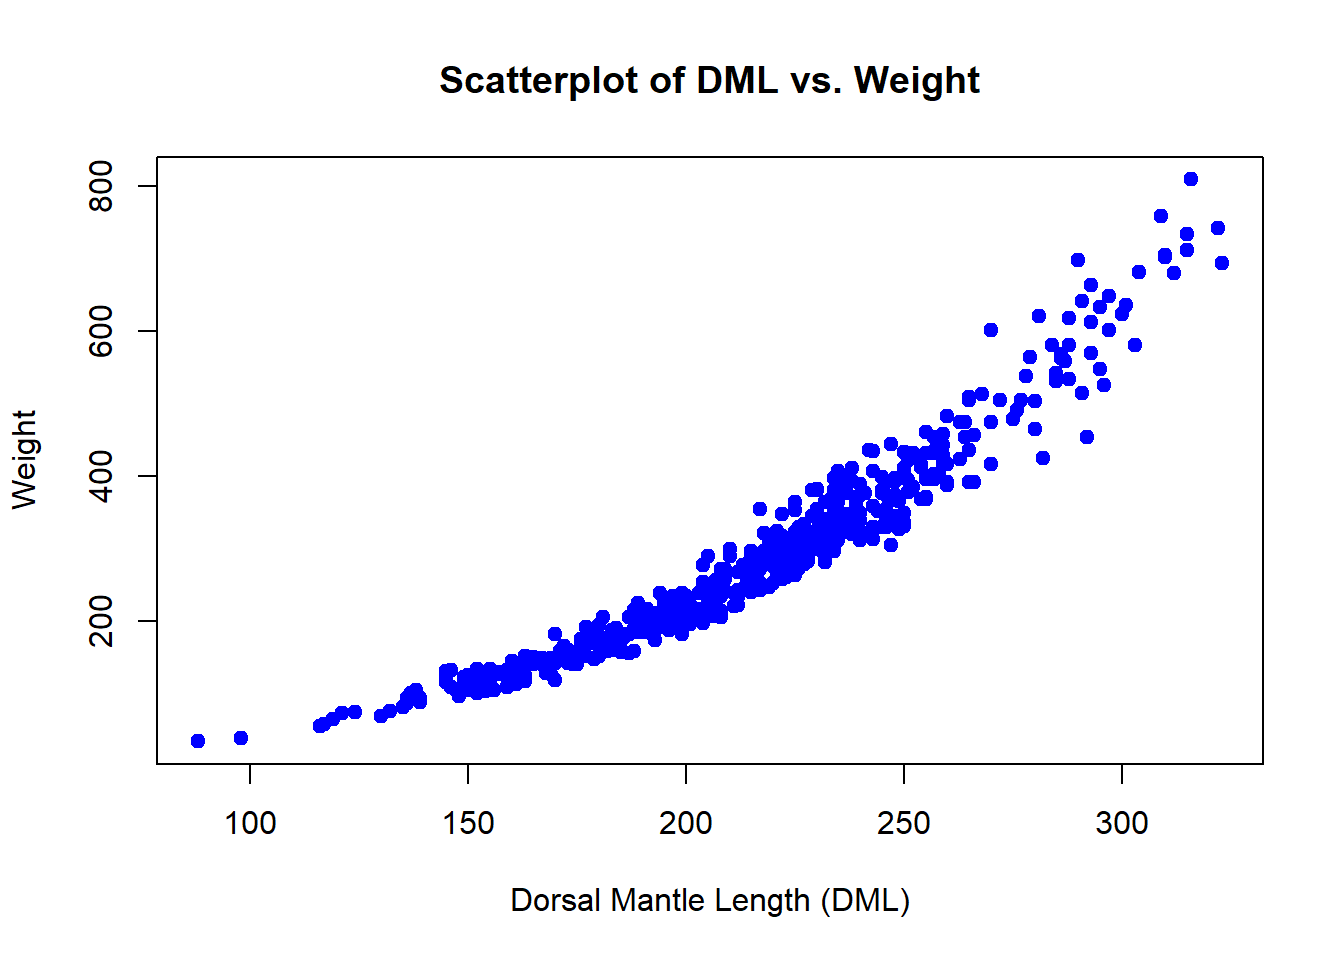
\includegraphics{exercise-4_lolavanuden_files/figure-latex/unnamed-chunk-9-1.pdf}

\begin{Shaded}
\begin{Highlighting}[]
\CommentTok{\#the curve is exponential therefore transformation is useful}
\end{Highlighting}
\end{Shaded}

\begin{Shaded}
\begin{Highlighting}[]
\NormalTok{squid}\SpecialCharTok{$}\NormalTok{log\_weight }\OtherTok{\textless{}{-}} \FunctionTok{log}\NormalTok{(squid}\SpecialCharTok{$}\NormalTok{weight)    }
\NormalTok{squid}\SpecialCharTok{$}\NormalTok{sqrt\_weight }\OtherTok{\textless{}{-}} \FunctionTok{sqrt}\NormalTok{(squid}\SpecialCharTok{$}\NormalTok{weight) }
\end{Highlighting}
\end{Shaded}

\begin{Shaded}
\begin{Highlighting}[]
\FunctionTok{plot}\NormalTok{(squid}\SpecialCharTok{$}\NormalTok{DML, squid}\SpecialCharTok{$}\NormalTok{log\_weight, }
     \AttributeTok{xlab =} \StringTok{"Dorsal Mantle Length (DML)"}\NormalTok{, }
     \AttributeTok{ylab =} \StringTok{"Log(Weight)"}\NormalTok{, }
     \AttributeTok{main =} \StringTok{"Scatterplot of DML vs. Log(Weight)"}\NormalTok{,}
     \AttributeTok{pch =} \DecValTok{19}\NormalTok{, }\AttributeTok{col =} \StringTok{"red"}\NormalTok{)}
\end{Highlighting}
\end{Shaded}

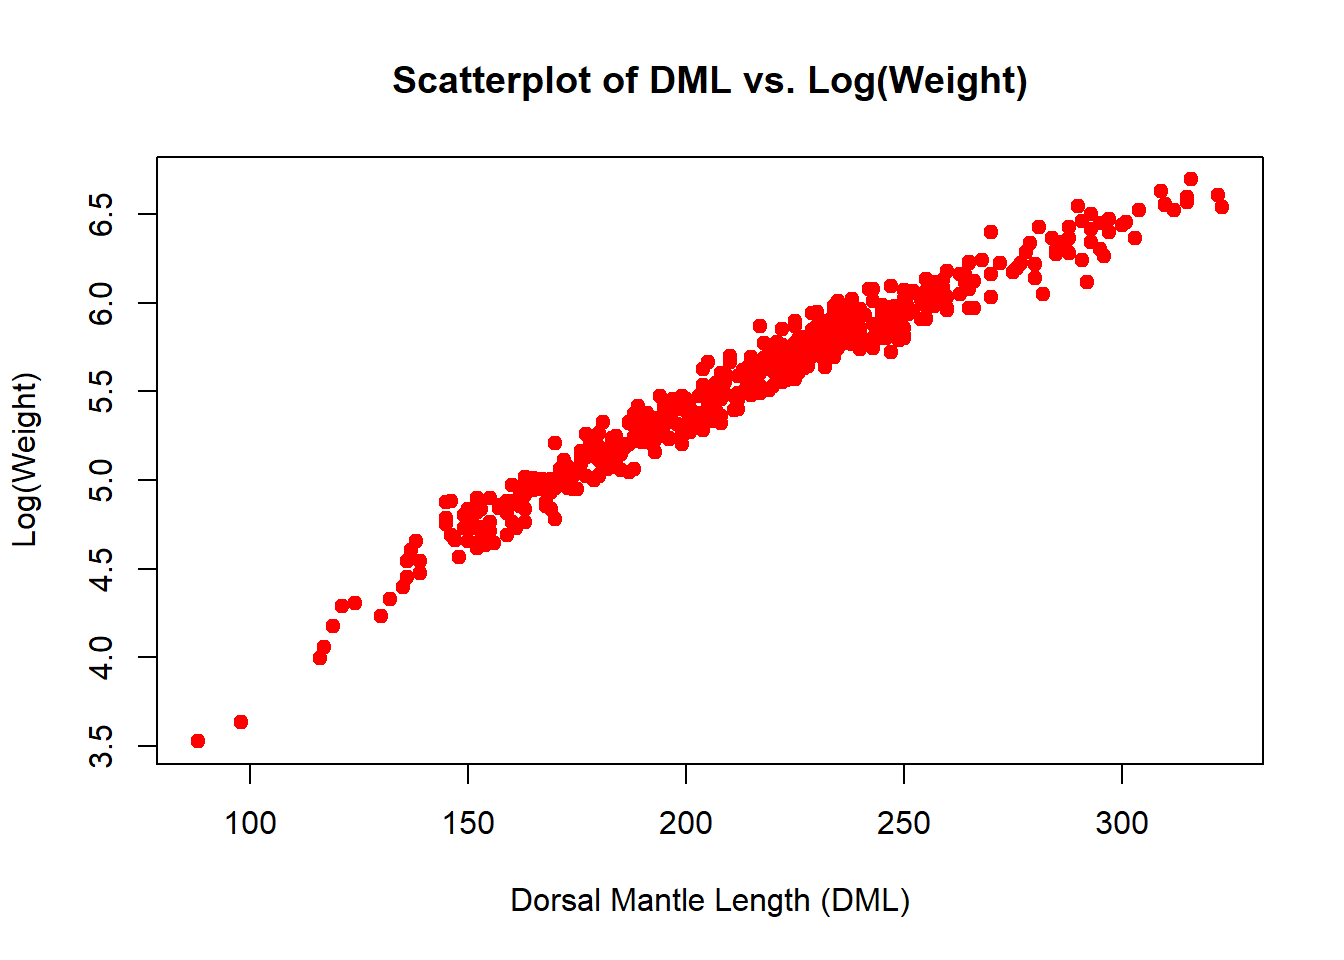
\includegraphics{exercise-4_lolavanuden_files/figure-latex/unnamed-chunk-11-1.pdf}

\begin{Shaded}
\begin{Highlighting}[]
\FunctionTok{plot}\NormalTok{(squid}\SpecialCharTok{$}\NormalTok{DML, squid}\SpecialCharTok{$}\NormalTok{sqrt\_weight, }
     \AttributeTok{xlab =} \StringTok{"Dorsal Mantle Length (DML)"}\NormalTok{, }
     \AttributeTok{ylab =} \StringTok{"Sqrt(Weight)"}\NormalTok{, }
     \AttributeTok{main =} \StringTok{"Scatterplot of DML vs. Sqrt(Weight)"}\NormalTok{,}
     \AttributeTok{pch =} \DecValTok{19}\NormalTok{, }\AttributeTok{col =} \StringTok{"green"}\NormalTok{)}
\end{Highlighting}
\end{Shaded}

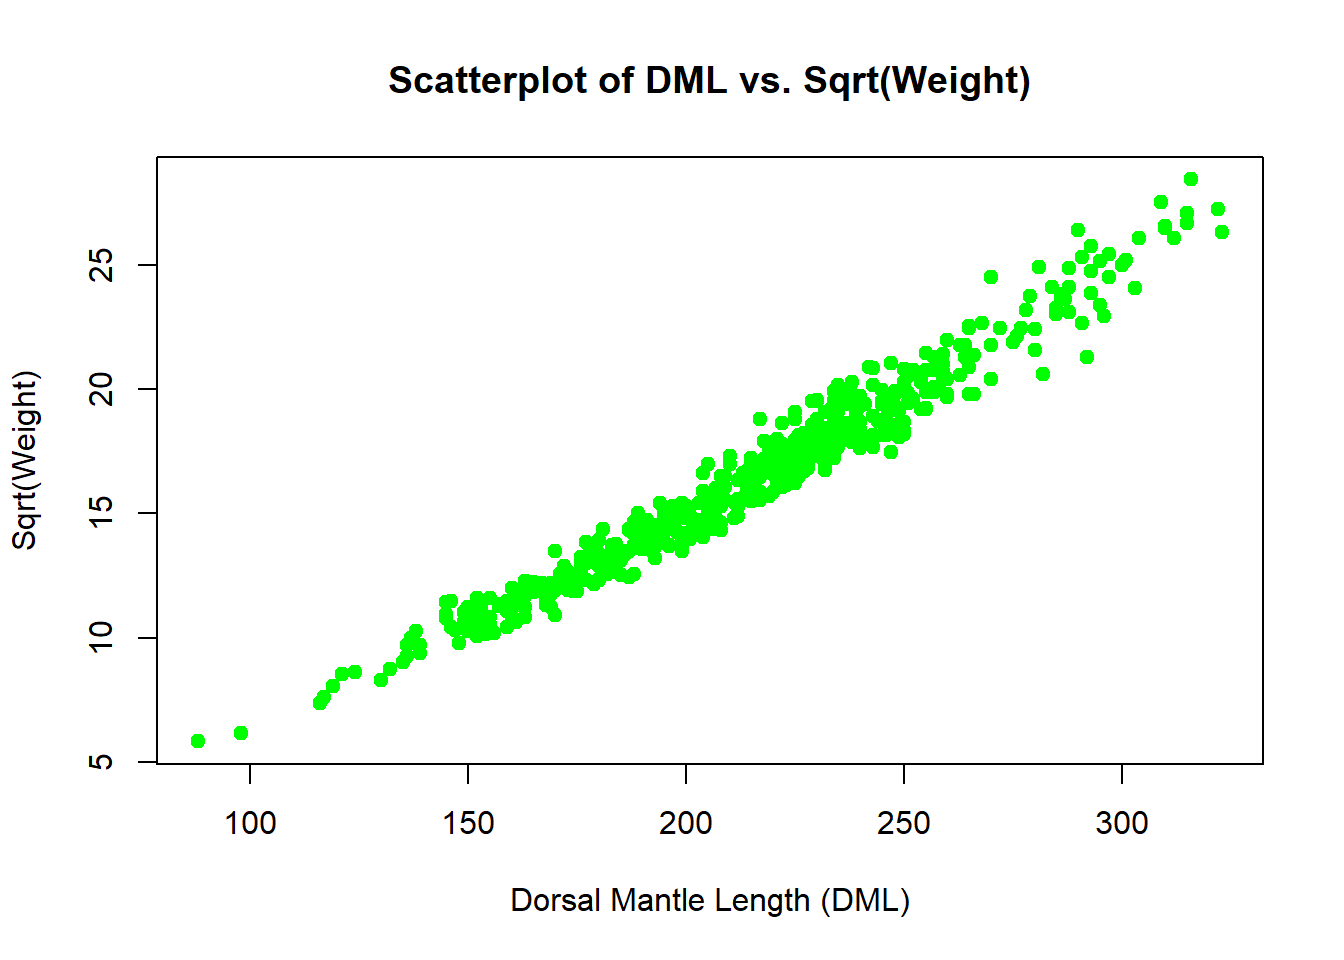
\includegraphics{exercise-4_lolavanuden_files/figure-latex/unnamed-chunk-12-1.pdf}

\begin{Shaded}
\begin{Highlighting}[]
\CommentTok{\#the sqrt plot best straightens the data}
\end{Highlighting}
\end{Shaded}

\begin{Shaded}
\begin{Highlighting}[]
\FunctionTok{png}\NormalTok{(}\StringTok{"DML\_vs\_Weight.png"}\NormalTok{, }\AttributeTok{width =} \DecValTok{800}\NormalTok{, }\AttributeTok{height =} \DecValTok{600}\NormalTok{)}
\FunctionTok{plot}\NormalTok{(squid}\SpecialCharTok{$}\NormalTok{DML, squid}\SpecialCharTok{$}\NormalTok{weight, }\AttributeTok{main =} \StringTok{"DML vs. Weight"}\NormalTok{)}
\FunctionTok{dev.off}\NormalTok{()}
\end{Highlighting}
\end{Shaded}

\begin{verbatim}
## pdf 
##   2
\end{verbatim}

\begin{Shaded}
\begin{Highlighting}[]
\FunctionTok{boxplot}\NormalTok{(squid}\SpecialCharTok{$}\NormalTok{DML }\SpecialCharTok{\textasciitilde{}}\NormalTok{ squid}\SpecialCharTok{$}\NormalTok{maturity.stage, }
        \AttributeTok{xlab =} \StringTok{"Maturity Stage"}\NormalTok{, }
        \AttributeTok{ylab =} \StringTok{"Dorsal Mantle Length (DML)"}\NormalTok{, }
        \AttributeTok{main =} \StringTok{"Boxplot of DML by Maturity Stage"}\NormalTok{,}
        \AttributeTok{col =} \FunctionTok{c}\NormalTok{(}\StringTok{"lightblue"}\NormalTok{, }\StringTok{"lightgreen"}\NormalTok{, }\StringTok{"lightpink"}\NormalTok{),}
        \AttributeTok{border =} \StringTok{"black"}\NormalTok{,}
        \AttributeTok{notch =} \ConstantTok{TRUE}\NormalTok{)}
\end{Highlighting}
\end{Shaded}

\begin{verbatim}
## Warning in (function (z, notch = FALSE, width = NULL, varwidth = FALSE, : some
## notches went outside hinges ('box'): maybe set notch=FALSE
\end{verbatim}

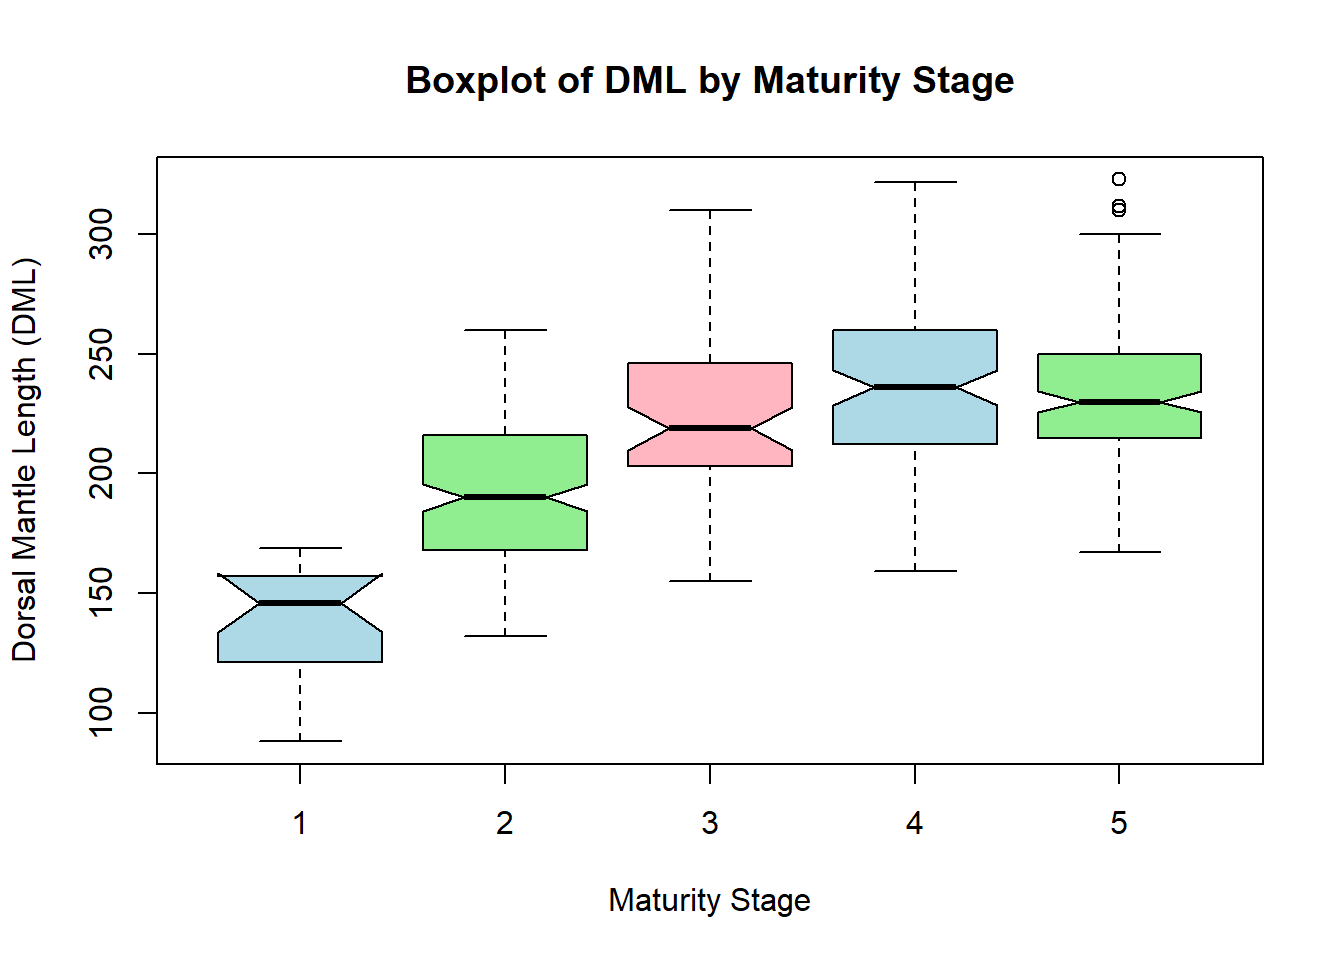
\includegraphics{exercise-4_lolavanuden_files/figure-latex/unnamed-chunk-14-1.pdf}

\begin{Shaded}
\begin{Highlighting}[]
\FunctionTok{pairs}\NormalTok{(squid[, }\FunctionTok{c}\NormalTok{(}\StringTok{"DML"}\NormalTok{, }\StringTok{"weight"}\NormalTok{, }\StringTok{"eviscerate.weight"}\NormalTok{, }\StringTok{"ovary.weight"}\NormalTok{, }\StringTok{"nid.length"}\NormalTok{, }\StringTok{"nid.weight"}\NormalTok{)])}
\end{Highlighting}
\end{Shaded}

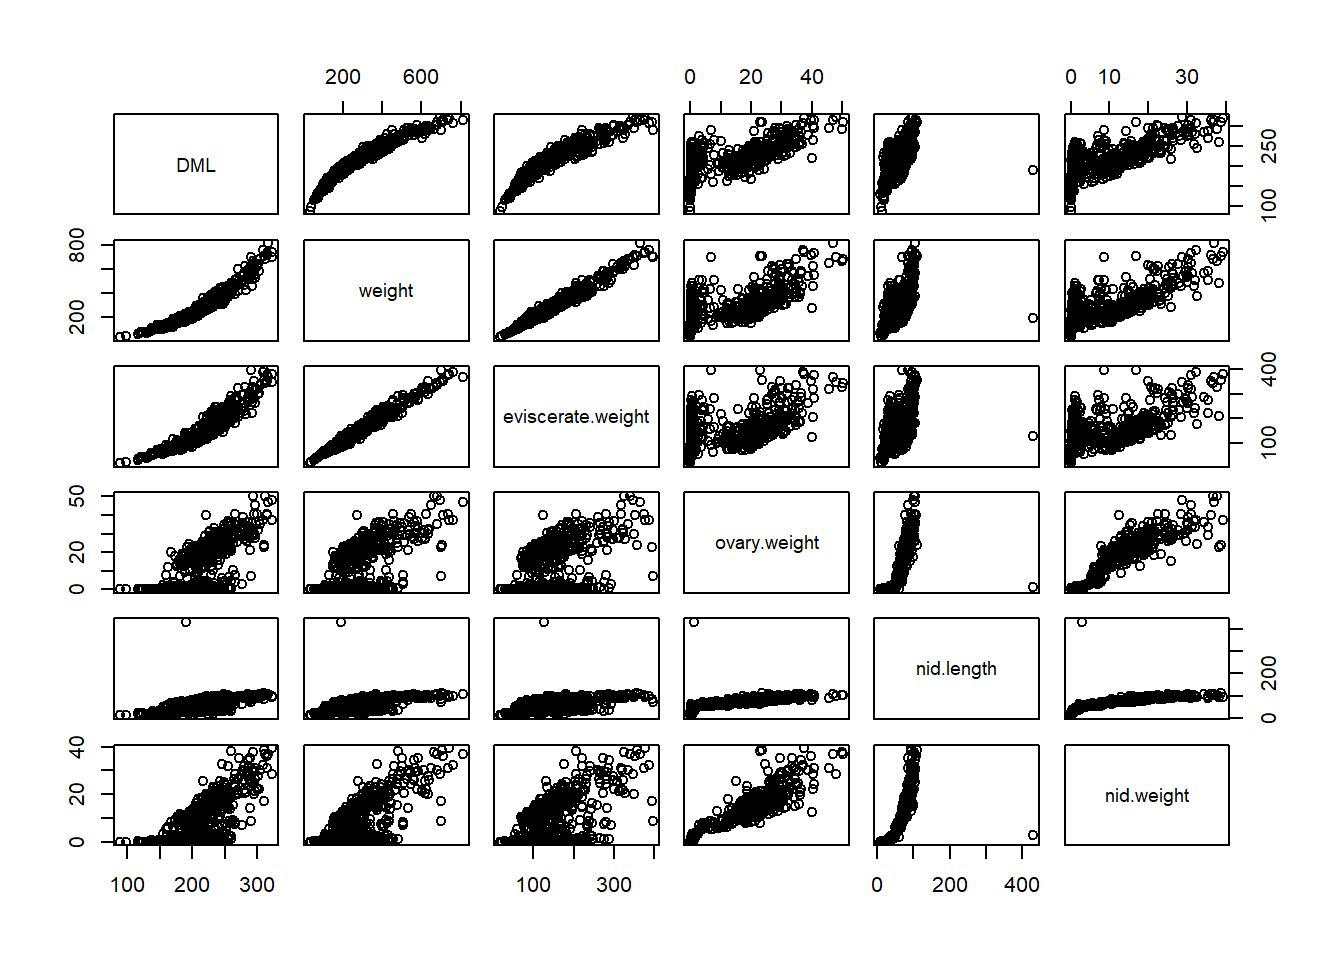
\includegraphics{exercise-4_lolavanuden_files/figure-latex/unnamed-chunk-15-1.pdf}

\end{document}
